	Na inicialização do projeto foi utilizado uma adaptação da técnica \textit{Inception Deck}, usada em metodologias ágeis, para a escrita do “termo” de abertura do projeto. Ela tem como objetivo estabelecer uma visão comum, entre todos os \textit{stakeholders}, sobre o que é o software, o que ele se dispõe a fazer. 

\subsection{Inception Deck - Projeto de Software}

	O \textit{Inception Deck} é composto por 10 seções que permitem alinhar as expectativas dos usuários quanto ao software que será desenvolvido. As seções são respectivamente: 1. Porque desenvolver o software; 2. Idealização do projeto; 3. Apresentação do Produto; 4. Definição do escopo do produto; 5. Usuários; 6. Arquitetura do produto; 7. Dificuldades do Projeto; 8. Tamanho do projeto; 9. Prioridades do projeto(tempo, custo, escopo) e 10. Definição do tempo e custo. Para se ajustar as necessidades do projeto as seções 8, 9 e 10 serão tratadas em apenas uma seção.


\textbf{Porque desenvolver o software}

	Esse seção elucida sobre as principais motivações que levaram ao desenvolvimento desse software.

	O software em desenvolvimento surgiu da necessidade de se obter uma  interface, na qual, o usuário pudesse interagir com uma bancada de teste de amortecedores. Suas principais funções consistem em configurar as informações necessárias para a execução dos testes, e a apresentação dos resultados em formato de relatório.


\textbf{Idealização e Escopo do projeto}

	Essa seção tem como objetivo caracterizar o software em desenvolvimento com o auxílio do \textit{framework} a seguir, e delimitar o escopo do produto, apresentando o que ele pretende fazer e o que ele não pretende.


	O software está sendo desenvolvido:
	\begin{itemize}
		\item \textbf{Para} Acadêmicos (Alunos e Professores) da Engenharia Automotiva
		\item \textbf{Que} precisam realizar testes em amortecedores de veículos leves
		\item \textbf{O} software em desenvolvimento
		\item \textbf{É} um aplicativo wep/app
		\item \textbf{Que} é responsável por fornecer os resultados do teste, em formato de relatório com gráficos específicos, após o mesmo ter sido configurado
		\item \textbf{Diferente de} soluções que não apresentam um resultado final em formato de relatório
		\item \textbf{Nosso produto} permite configurar vários tipos de testes de amortecedores, bem como, manter um histórico dos testes realizadas e amortecedores testados.
	\end{itemize}

	Escopo do produto:
	
	% Lembrar o povo de incluir essa biblioteca --->>>>>> \usepackage{booktabs}
	\begin{table}[!h]
		\centering
		\caption{Escopo do software em desenvolvimento}
		\label{escopo}
		\begin{tabular}{cc}
		\hline
		\rowcolor[HTML]{C0C0C0} 
		{\color[HTML]{000000} \textbf{Dentro do Escopo}} & {\color[HTML]{000000} \textbf{Fora do Escopo}} \\ \hline
		{\color[HTML]{000000} \begin{tabular}[c]{@{}c@{}}Fornecer uma interface entre o\\  usuário e a bancada\end{tabular}} & {\color[HTML]{000000} \begin{tabular}[c]{@{}c@{}}Fornecer comparação entre\\  os amortecedores\end{tabular}} \\ \hline
		{\color[HTML]{000000} \begin{tabular}[c]{@{}c@{}}Realizar a seleção e\\ configuração do teste\end{tabular}} & {\color[HTML]{000000} \begin{tabular}[c]{@{}c@{}}Realizar a simulação de um teste\\  apenas pelo software da bancada\end{tabular}} \\ \hline
		{\color[HTML]{000000} \begin{tabular}[c]{@{}c@{}}Apresentar os resultados do teste\\ num formato de relatório\end{tabular}} & {\color[HTML]{000000} } \\ \hline
		\end{tabular}
	\end{table}


\textbf{Usuários}

	Esse seção define toda comunidade possivelmente interessada no software, o que inclui, tanto os desenvolvedores, quanto acadêmicos, além de pessoas de outras áreas.

	\begin{figure}[h]
		\centering
		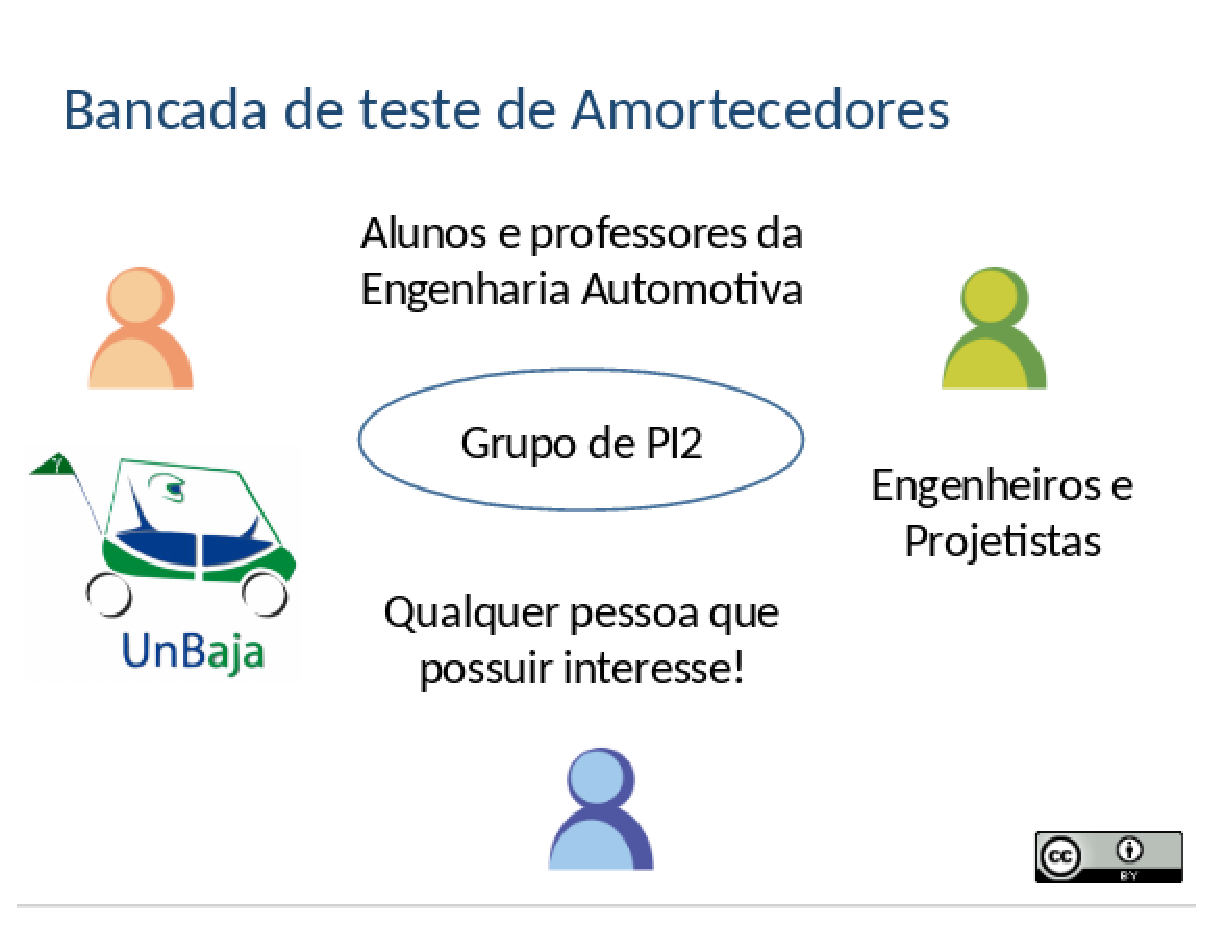
\includegraphics[width=0.8\textwidth]{resource/usuarios.eps}
		\caption{Comunidade de usuários do software}
		\label{img:usuarios}
	\end{figure}


\textbf{Arquitetura do produto}

	Essa seção é responsável por apresentar a arquitetura definida pelo time de desenvolvimento, bem como, descrever o suporte tecnológico.

	% TODO - atualizar
	A arquitetura de software será modelada em três camadas distintas, mas que estabelecem uma comunicação entre si. Esta estratégia foi adotada por permitir a modularização entre as camadas, pois apesar de uma camada necessitar da outra para o funcionamento total do bancada, será possível executar os testes de sistema separadamente em cada camada. Assim, os problemas encontrados em uma camada podem ser resolvidos facilmente sem necessariamente afetar as demais. A imagem \ref{arquiteturaSOFT} apresenta o diagrama da arquitetura estabelecida.

	\begin{figure}[h]
		\centering
		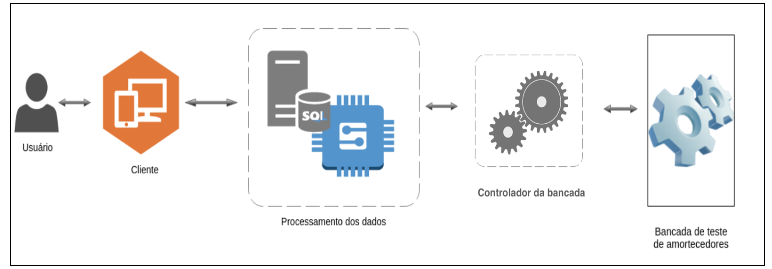
\includegraphics[width=1\textwidth]{arquiteturaSOFT}
		\caption{Arquitetura do Projeto de Software}
		\label{arquiteturaSOFT}
	\end{figure}

	O software será dividido em 3 camadas:
	Cliente;
	Processamento dos Dados e;
	Controlador da Bancada.

	A equipe de Engenharia de Software ficará responsável por implementar os módulos 1 e 2 e a equipe de Engenharia Eletrônica ficará responsável por implementar o módulo 3.

	\textbf{Modulo 1}

	O primeiro módulo, cliente, será responsável por realizar as operações, por meio das funcionalidades desenvolvidas, para a execução e controle da bancada. Para isso, será desenvolvida uma aplicação \textit{web-app} o qual será embarcada no microcontrolador e assim, ausenta a necessita do usuário final ter um aplicativo específico para interagir com o sistema, sendo necessário apenas um \textit{browser} a partir de um dispositivo que permita conexão via wi-fi. Este primeiro módulo será desenvolvido utilizando a linguagem Python v.3.4.3 utilizando \textit{framework} Django v.1.9. 

	Apesar do Django apresentar um arquitetura própria baseado no MVC (Model-View-Controller), o \textit{framework} permite a inserção de padrões de software sobre a medida do desenvolver conforme suas necessidades.

	\textbf{Modulo 2}

	O segundo módulo será responsável por estabelecer a comunicação entre o APP e o Microcontrolador. Além disso, ele fará o tratamento adequada dos dados oriundos dos sensores da bancada. Este tratamento está relacionado à forma como os dados são fornecidos a partir do microcontrolado. Os dados serão disponibilizados pelo módulo três por meio de uma conexão Wi-Fi.

	A base de dados que será utilizada é o PostgreSQL por ser uma ferramenta de fácil utilização, escalável e gratuita. E o módulo será desenvolvido, em sua totalidade, em Python v.3.4.3.


	\textbf{Modulo 3}

	Já o terceiro módulo tem a responsabilidade de gerir o controle dos dados de entrada e saída da bancada. Ou seja, ele é incumbido de receber e repassar as informações que chegam dos sensores e também acionar na bancada as informações fornecidas pelo software. Este módulo, especificamente, será desenvolvido pela equipe da engenharia eletrônica. Para este módulo a principal linguagem utilizada será o ANSI C.


	A imagem a seguir, \ref{img:modulos}, ilustra os relacionamentos das três camadas sobre uma perspectiva mais detalhada.

	\begin{figure}[h]
		\centering
		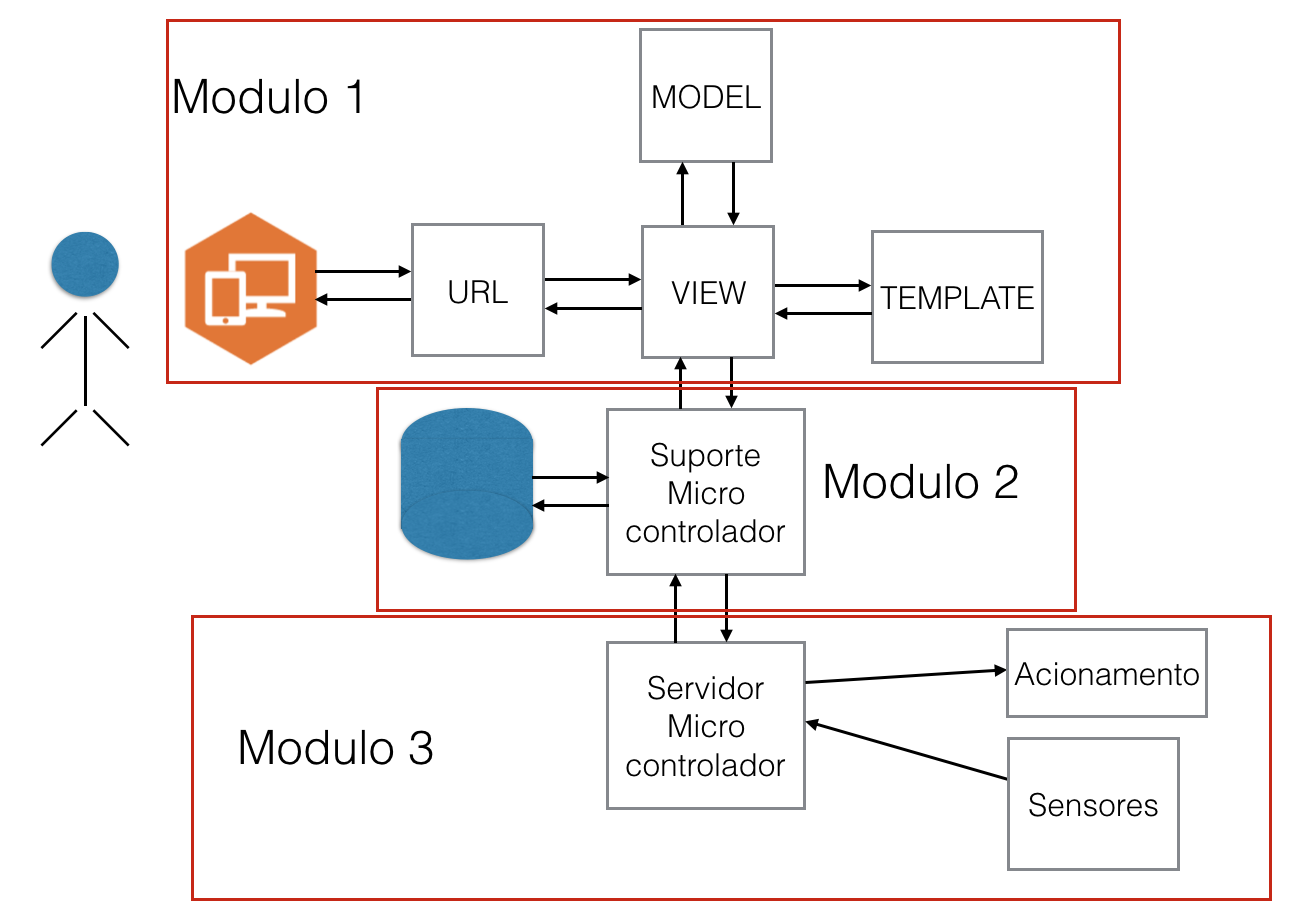
\includegraphics[width=0.8\textwidth]{resource/modulos.png}
		\caption{Diagrama representativo da arquitetura proposta}
		\label{img:modulos}
	\end{figure}

	O cliente, a partir de uma camada de mapeamento de URL para TEMPLATE, requisitará uma página web. A URL terá o papel de associar a página requisitada a uma VIEW que posteriormente montará a página web a partir dos objetos (modelos) provindos da camada MODEL e das validações geridas pela camada TEMPLATE. A camada VIEW fará a comunicação com o suporte ao microcontrolador que por sua vez, estabelece a comunicação com a base de dados PostgreSQL. A camada onde encontra-se o microcontrolador receberá os comandos de acionamento da bancada a partir do módulo de suporte e também encaminhará para este módulo os resultados coletados pelos sensores.

\textbf{Dificuldades do Projeto}

	A Tabela \ref{tab:risco} lista as dificuldades idenficadas em forma de risco e as ações necessárias para mitigá-las.

	\begin{table}[h]
	\centering
	\caption{Risco para o Desenvolvimento do Software}
	\label{tab:risco}
	\resizebox{\textwidth}{!}{%
	\begin{tabular}{@{}ll@{}}
	\toprule
	\multicolumn{1}{c}{\textbf{Riscos}}                                   & \multicolumn{1}{c}{\textbf{Ações}}                                                \\ \midrule
	\multicolumn{1}{|l|}{Equipe não evoluir no desenvolvimento do App}    & \multicolumn{1}{l|}{Replanejar o escopo e promover um número maior de pareamento} \\ \midrule
	\multicolumn{1}{|l|}{Algum membro sem experiência na tecnologia}      & \multicolumn{1}{l|}{Realizar dojo para alinhamento do conhecimento}               \\ \midrule
	\multicolumn{1}{|l|}{Dificuldade para realizar reuniões presenciais}  & \multicolumn{1}{l|}{Realizar reunião on-line via Hangouts}                        \\ \midrule
	\multicolumn{1}{|l|}{Mudança muito grande dos requisitos do sistemas} & \multicolumn{1}{l|}{Priorizar histórias de usuário e redefinir escopo}            \\ \midrule
	\multicolumn{1}{|l|}{Descontinuidade de alguma biblioteca importante} & \multicolumn{1}{l|}{Repriorizar as tecnologias}                                   \\ \bottomrule
	\end{tabular}%
	}
	\end{table}

\textbf{Roadmap} 
\label{subsec:roadmap}

	Essa seção apresenta uma visão das funcionalidades presentes no software e quando elas serão entregues.

	\begin{figure}[h]
		\centering
		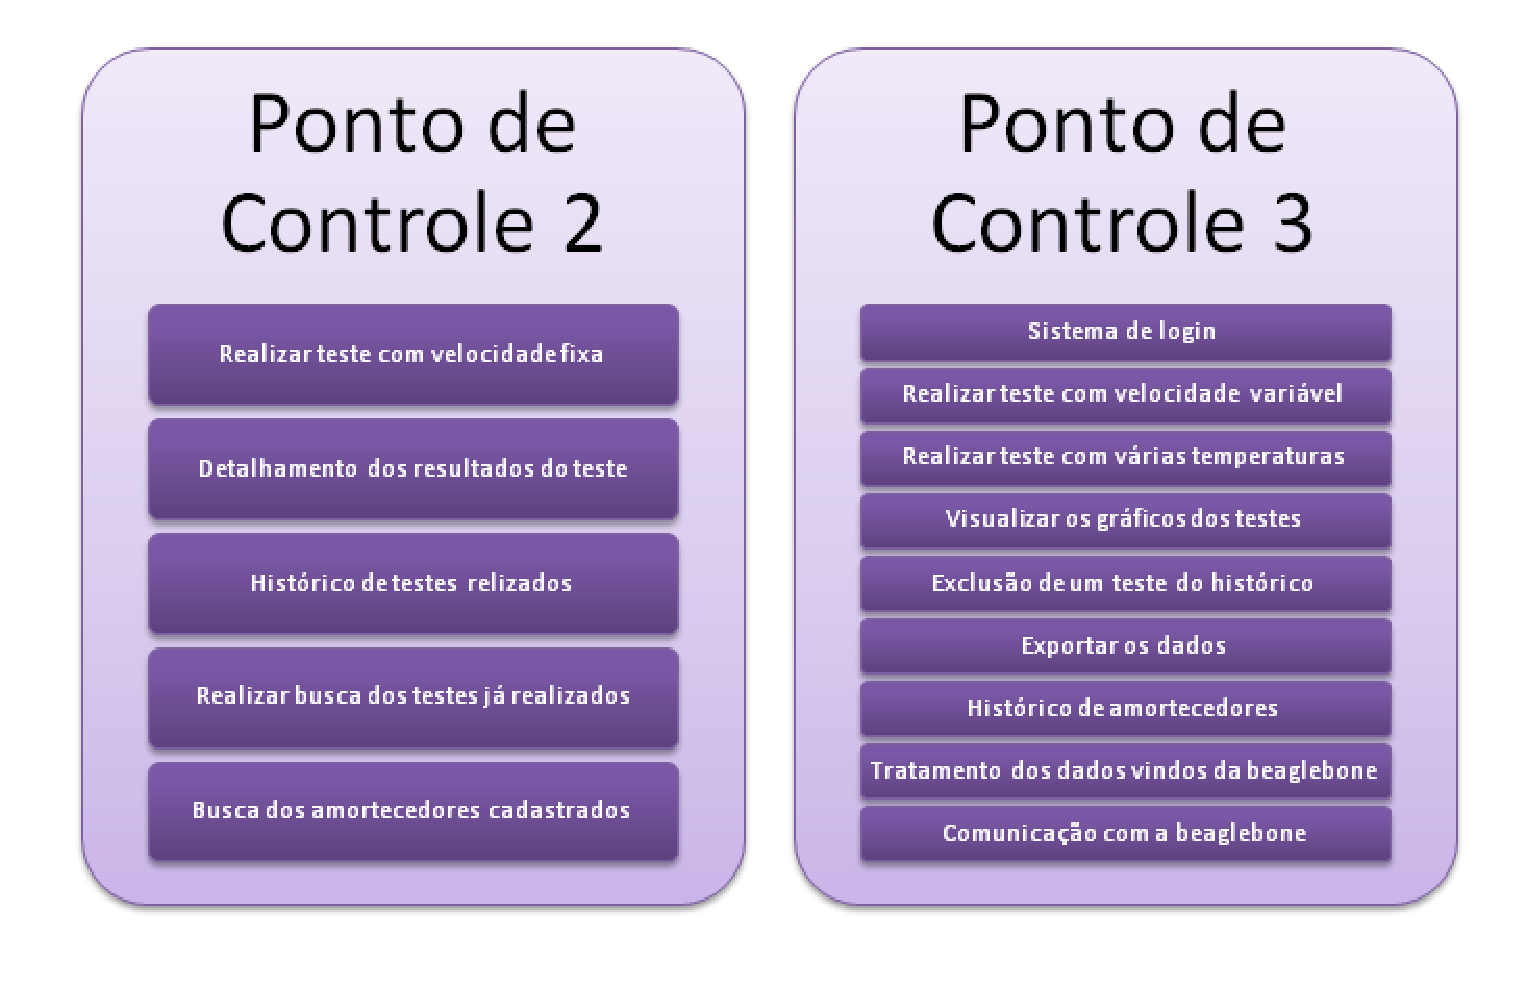
\includegraphics[width=1\textwidth]{resource/roadmap.eps}
		\caption{Funcionalidades previstas}
		\label{img:usuarios}
	\end{figure}


\subsection{Ponto de Controle II}
\subsubsection{Processo de Desenvolvimento}

	Com o objetivo de gerenciar o fluxo de desenvolvimento (implementação, teste unitário e teste de aceitação), adotou-se o uso do \textit{plugin} Zenhub. Este é instalado no \textit{browser}, ele altera a apresentação do site responsável por armazenar as versões do software, no caso desse trabalho o GitHub. O Zenhub cria uma \textit{dashboard}, Figura \ref{img:zenHub},  onde é possível separar as atividades em \textit{boards}. A utilização desse \textit{plugin} permite centralizar todas as informações referentes ao software.

	\begin{figure}[h]
		\centering
		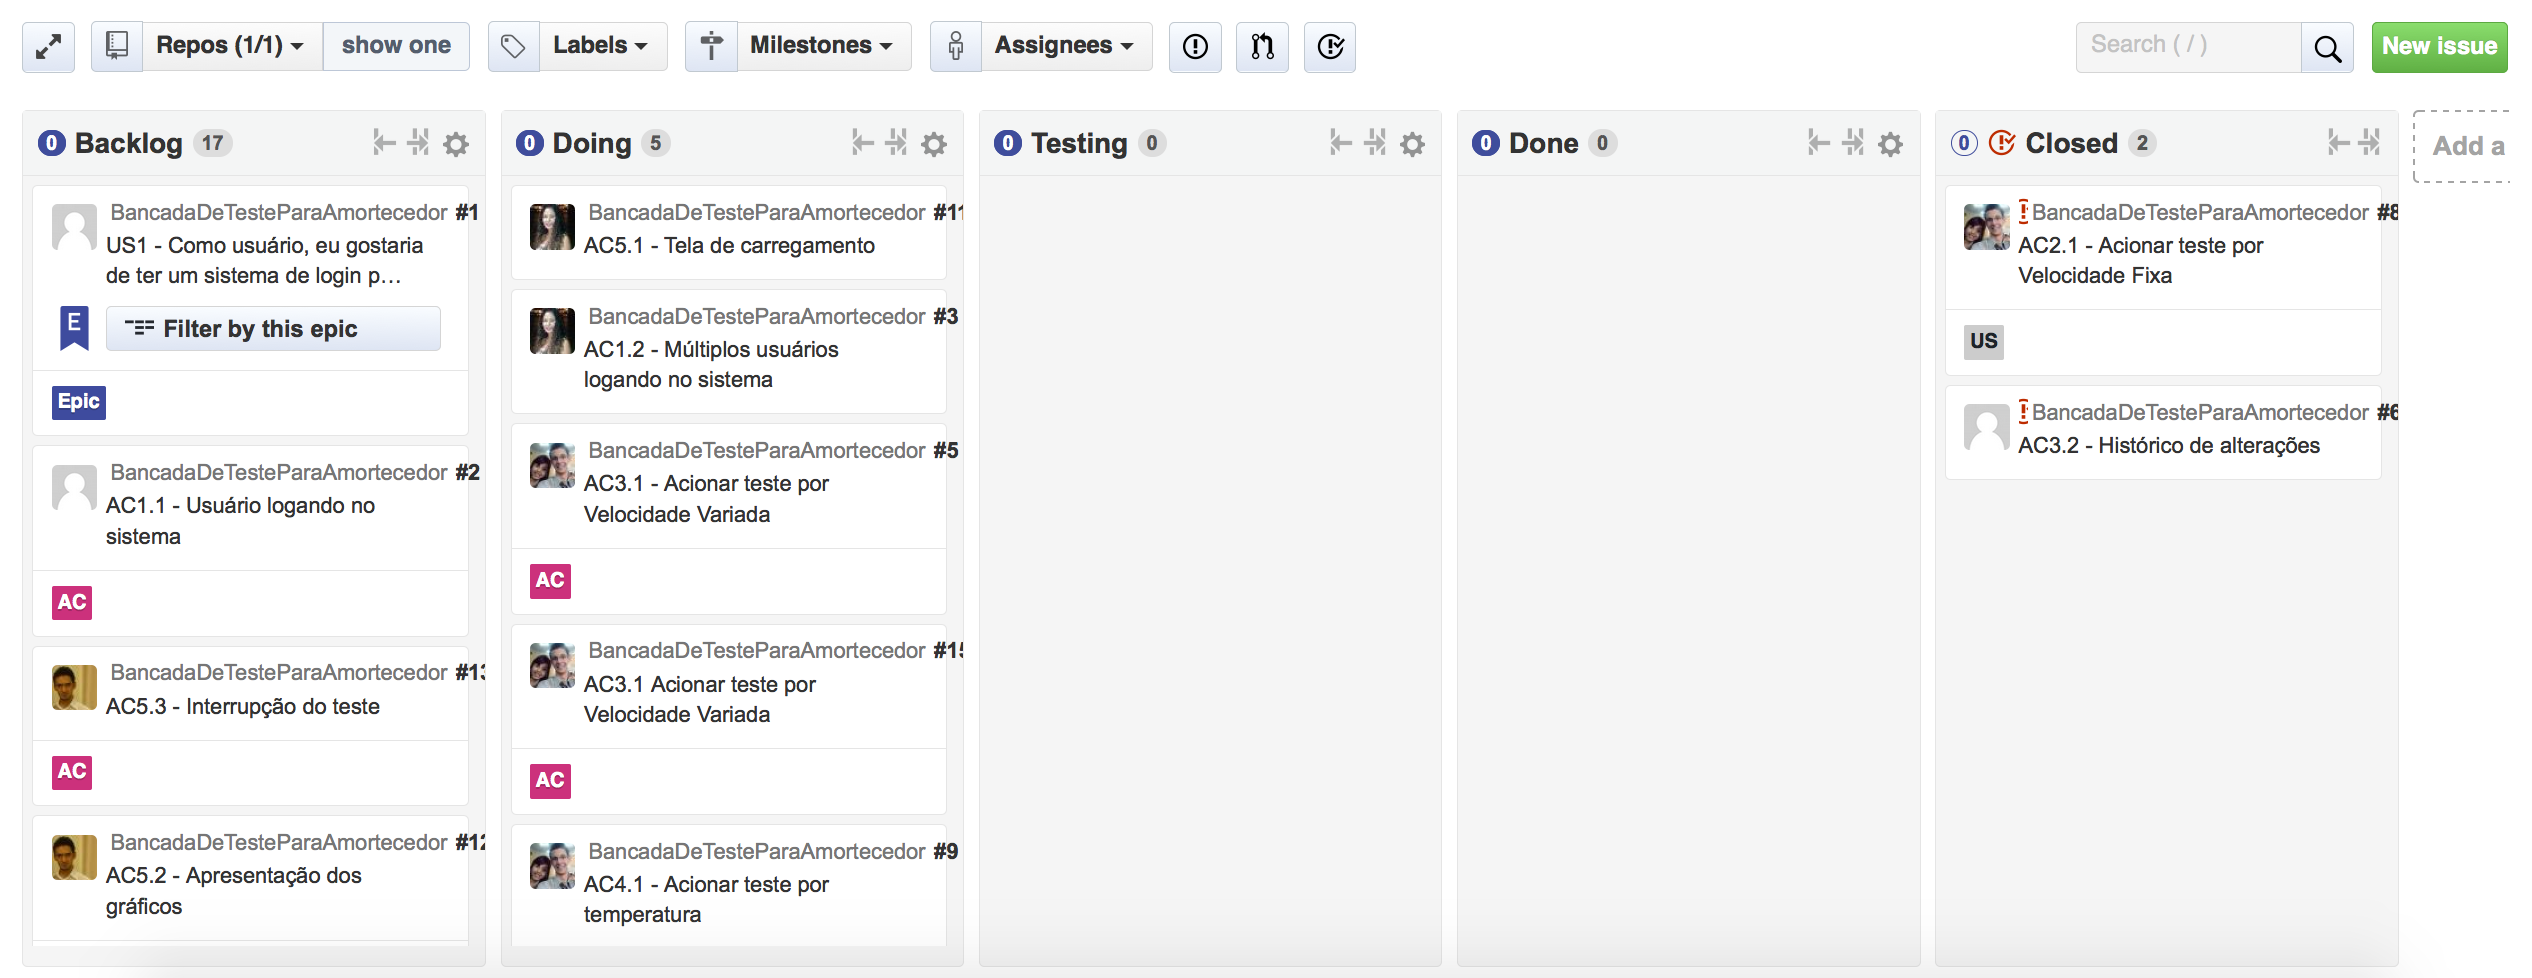
\includegraphics[width=1\textwidth]{resource/zenHub.png}
		\caption{Ferramenta para Gestão de Requisitos - ZenHub}
		\label{img:zenHub}
	\end{figure}


\subsubsubsection{Gerenciamento dos Requisitos}

	Os requisitos sofrerão constantes atualizações, principalmente no que tange a definição dos dados a serem monitoradas durante o experimento da bancada. Para tanto, adotou-se a técnica de escrita de histórias de usuário segundo as metodologias ágeis, a fim, de aceitar as mudanças e manter um recorrente acompanhamento do software em relação a mecânica da bancada.

	Os requisitos não-funcionais acompanharam as historias de usuário mapeadas para testes de aceitação. Acredita-se que a maior parte destes requisitos está ligada a usabilidade e confiabilidade, principalmente em relação à acurácia dos cálculos e plotagens de gráficos.

	Para a elicitação das histórias de usuário foi realizado reuniões com a cliente principal, Larissa, graduanda em Engenharia Automotiva na UnB. As histórias foram armazenas em \textit{issues} no GiHub. \textit{Issue} é uma funcionalidade do GitHub que permite que os desenvolvedores possam armazenar as tarefas referentes ao desenvolvimento do projeto.

	Após a elicitação, os requisitos foram reunidos no \textit{backlog} do projeto, tabela \ref{USsoft}, sendo esses, priorizados e divididos em duas iterações. As iterações representam os marcos: Ponto de Controle 2 e Ponto de Controle 3. Os entregáveis de cada iteração são descritos no \textit{roadmap} do produto, apresentado na seção \ref{subsec:roadmap}.

	\begin{table}[!h]
		\centering
		\caption{Histórias de Usuário}
		\label{USsoft}
		\resizebox{\textwidth}{!}{%
		\begin{tabular}{ll}
		\hline
		\multicolumn{2}{c}{\textbf{Backlog do Produto}} \\ \hline
		\multicolumn{1}{c}{\textbf{ID}} & \multicolumn{1}{c}{\textbf{Descrição}} \\ \hline
		US1 & \begin{tabular}[c]{@{}l@{}}Como usuário, eu gostaria de ter um sistema de login para que apenas o\\ usuário logado possa realizar o teste.\end{tabular} \\ \hline
		US2 & Como administrador, eu gostaria de realizar um teste com velocidades fixas \\ \hline
		US3 & Como administrador, eu gostaria de realizar um teste com velocidades variáveis \\ \hline
		US4 & Como administrador, eu gostaria de realizar um teste com várias temperaturas \\ \hline
		US5 & \begin{tabular}[c]{@{}l@{}}Como administrador, eu quero visualizar os gráficos do teste para ter acesso\\ aos resultados\end{tabular} \\ \hline
		US6 & \begin{tabular}[c]{@{}l@{}}Como administrador, eu desejo excluir um teste realizado para manter o \\ histórico limpo de testes indesejados.\end{tabular} \\ \hline
		US7 & \begin{tabular}[c]{@{}l@{}}Como usuário, eu gostaria de ver os dados detalhados do teste para ter \\ acesso a todas as informações referentes ao teste\end{tabular} \\ \hline
		US8 & Como usuário, eu gostaria de exportar os dados do teste para que eu possa imprimi-los \\ \hline
		US9 & \begin{tabular}[c]{@{}l@{}}Como usuário, eu gostaria de visualizar o histórico dos testes para visualizar a lista dos \\ experimentos já realizados na bancada.\end{tabular} \\ \hline
		US10 & \begin{tabular}[c]{@{}l@{}}Como usuário, gostaria de realizar uma busca dos testes realizados na bancada para \\ que eu tenha acesso de forma rápida\end{tabular} \\ \hline
		US11 & \begin{tabular}[c]{@{}l@{}}Como usuário, eu gostaria de visualizar um histórico dos amortecedores para que eu\\  possa visualizar os amortecedores já cadastrados\end{tabular} \\ \hline
		US12 & \begin{tabular}[c]{@{}l@{}}Como usuário, gostaria de realizar uma busca dos amortecedores cadastrados\\ para que eu tenha acesso de forma rápida\end{tabular} \\ \hline
		\end{tabular}%
		}
	\end{table}

	Os testes de aceitação serão apresentados em uma seção posterior. Os demais testes, unitário e funcional, serão desenvolvimentos apenas na segunda iteração (último ponto de controle).


\subsubsubsection{Protótipos do Software}

	Os protótipos foram modelados com base no levantamento inicial dos requisitos de software. O sistema inicialmente foi estruturado em cinco telas as quais são ilustradas a seguir.

	\begin{figure}[p]
		\centering
		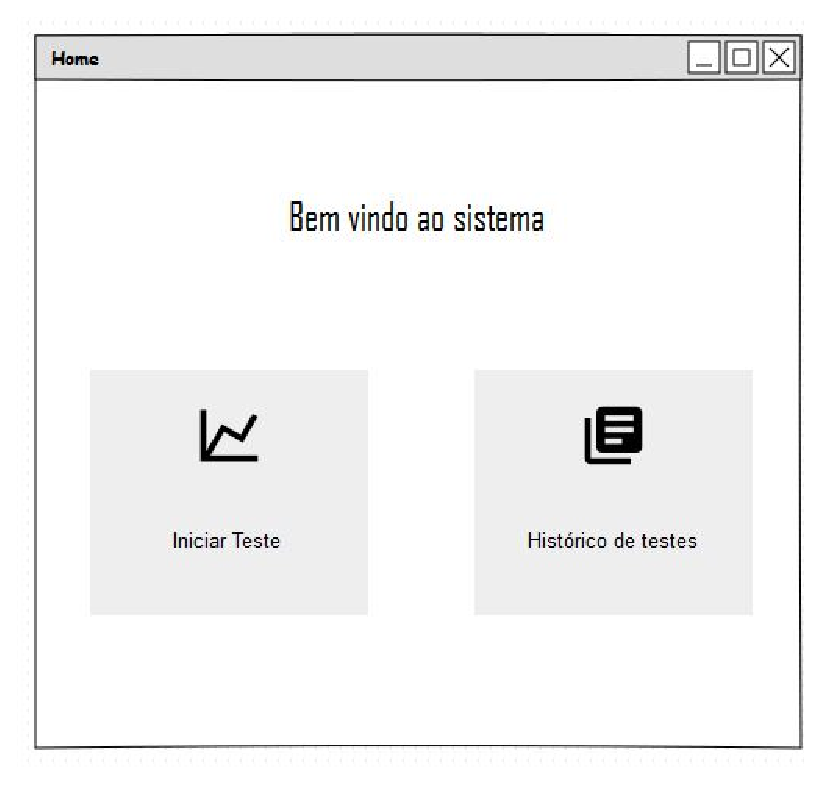
\includegraphics[width=0.6\textwidth]{resource/home.eps}
		\caption{Página inicial do sistema}
		\label{img:home}
	\end{figure}

	\begin{figure}[p]
		\centering
		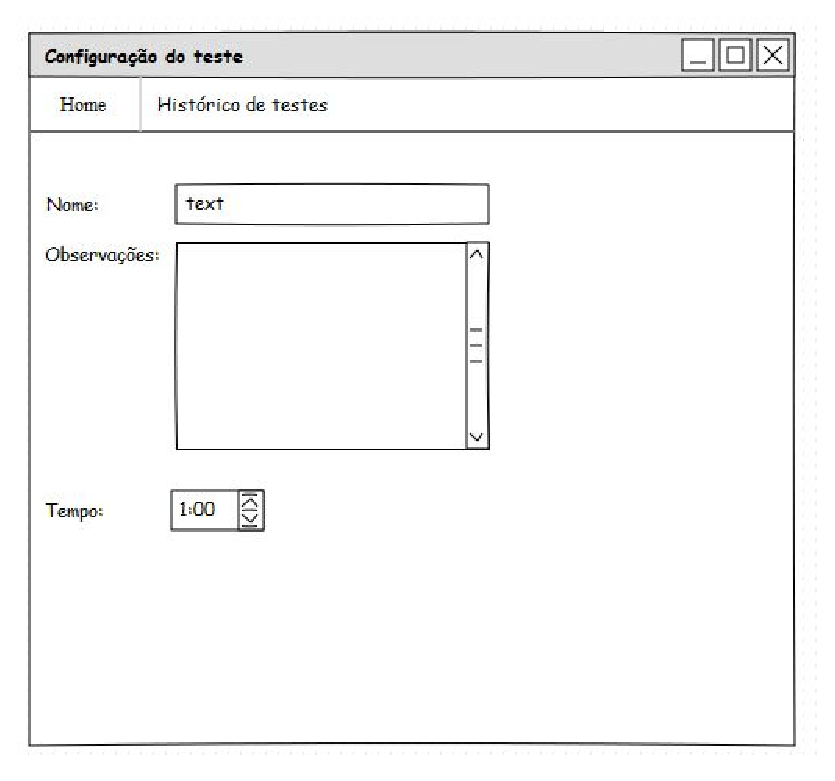
\includegraphics[width=0.6\textwidth]{resource/configteste.eps}
		\caption{Página de configuração do teste}
		\label{img:conf}
	\end{figure}
	
	\begin{figure}[p]
		\centering
		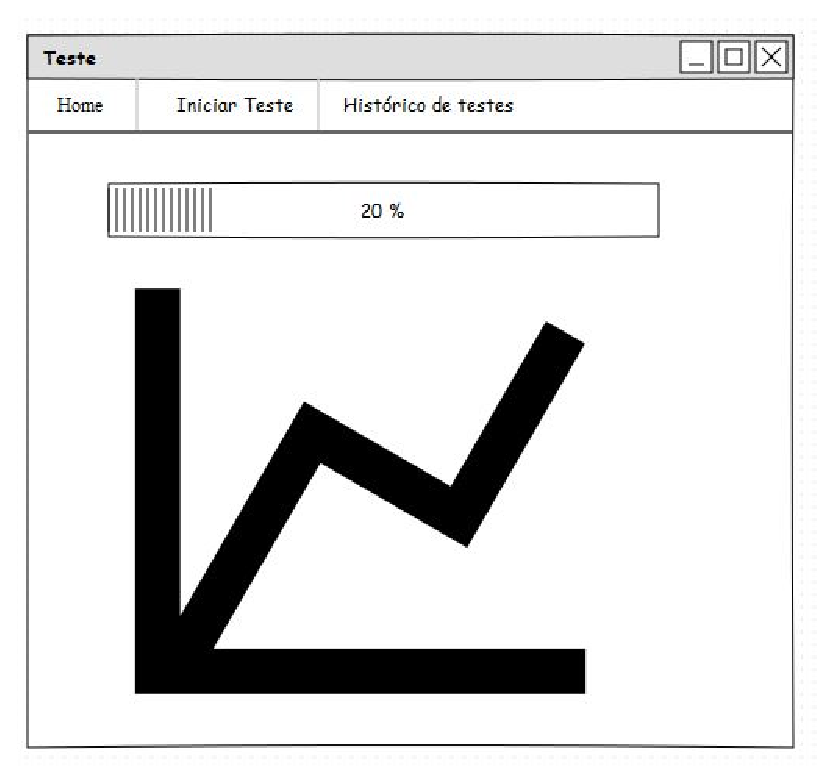
\includegraphics[width=0.6\textwidth]{resource/teste.eps}
		\caption{Realização do teste}
		\label{img:teste}
	\end{figure}

	\begin{figure}[p]
		\centering
		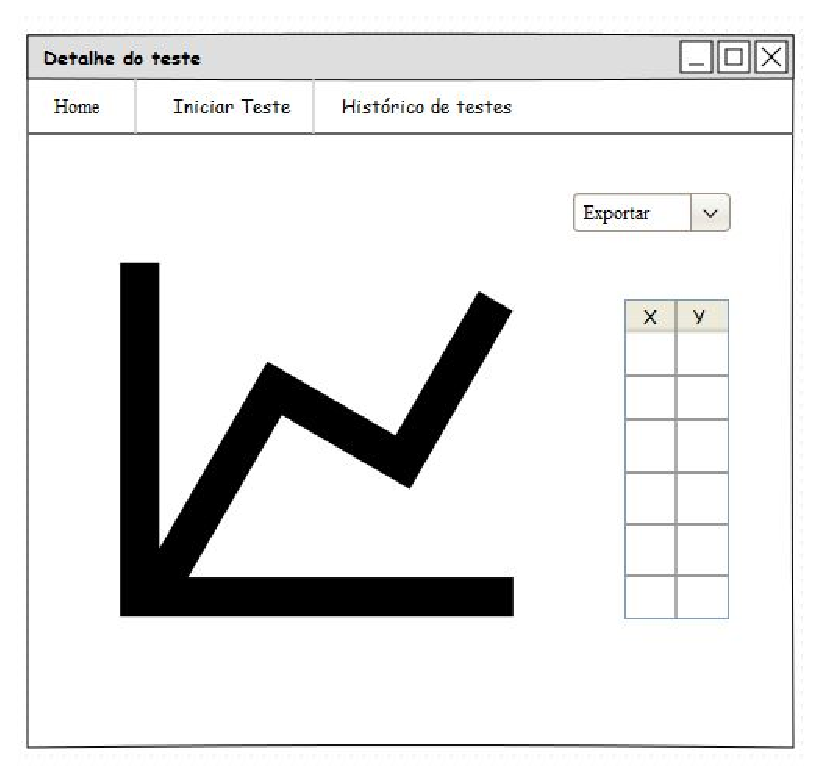
\includegraphics[width=0.6\textwidth]{resource/detalheteste.eps}
		\caption{Resultados dos testes}
		\label{img:detalhe}
	\end{figure}
	
	\begin{figure}[!h]
		\centering
		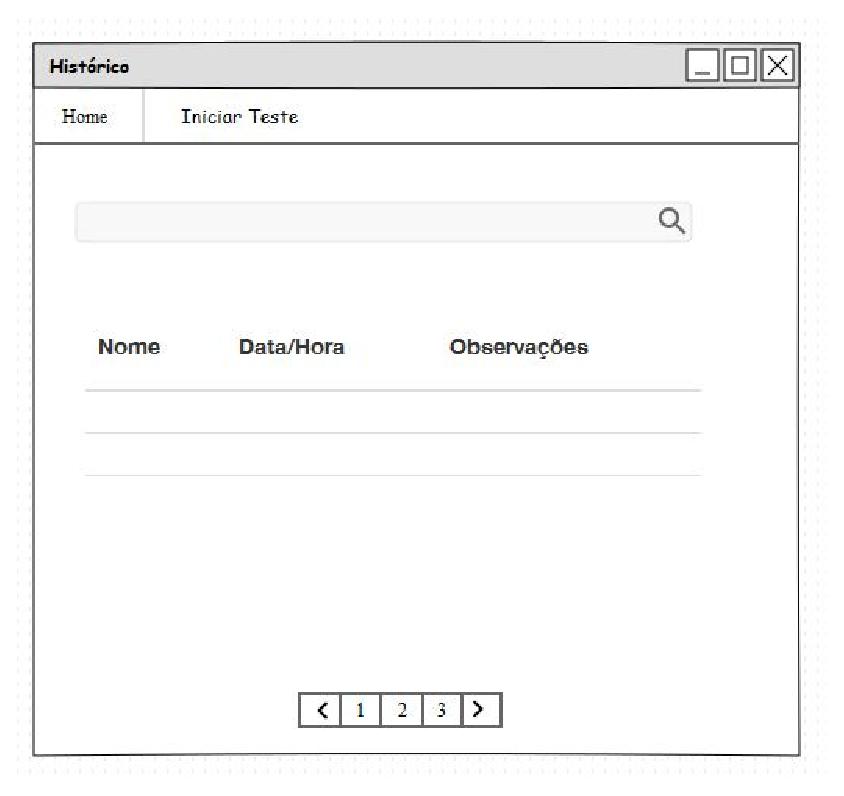
\includegraphics[width=0.6\textwidth]{resource/historico.eps}
		\caption{Histórico dos testes realizados}
		\label{img:historico}
	\end{figure}

\newpage
\subsubsubsection{Suporte Tecnológico}
	A Tabela \ref{tab:tech} apresenta as tecnologias que auxiliaram o desenvolvimento do projeto.
	\begin{table}[h]
	\centering
	\caption{Tecnologias utilizadas}
	\label{tab:tech}
	\begin{tabular}{ccc}
	\hline
	\textbf{Ferramenta}              & \textbf{Versão}                   & \textbf{Função}                                                   \\ \hline
	\multicolumn{1}{|c|}{Git}        & \multicolumn{1}{c|}{mais recente} & \multicolumn{1}{c|}{Controle de versão}                           \\ \hline
	\multicolumn{1}{|c|}{GitHub}     & \multicolumn{1}{c|}{mais recente} & \multicolumn{1}{c|}{Armazenamento das versões}                    \\ \hline
	\multicolumn{1}{|c|}{ZenHub}     & \multicolumn{1}{c|}{mais recente} & \multicolumn{1}{c|}{Gerenciamento do desenvolvimento}             \\ \hline
	\multicolumn{1}{|c|}{Python}     & \multicolumn{1}{c|}{3.4.3}        & \multicolumn{1}{c|}{Linguaguem de desenvolvimento}                \\ \hline
	\multicolumn{1}{|c|}{Django}     & \multicolumn{1}{c|}{1.9.5}        & \multicolumn{1}{c|}{Framework para desenvolvimento Web em Python} \\ \hline
	\multicolumn{1}{|c|}{PostgreSQL} & \multicolumn{1}{c|}{9.4.7}        & \multicolumn{1}{c|}{Base de dados}                                \\ \hline
	\multicolumn{1}{|c|}{Highcharts} & \multicolumn{1}{c|}{4.2.4}        & \multicolumn{1}{c|}{Plotagem dos gráficos}                        \\ \hline
	\multicolumn{1}{|c|}{Bootstrap}  & \multicolumn{1}{c|}{3.3.6}        & \multicolumn{1}{c|}{Padronização dos templates das páginas web}   \\ \hline
	\multicolumn{1}{|c|}{Xhtml2pdf}  & \multicolumn{1}{c|}{0.1}          & \multicolumn{1}{c|}{Gerar PDF dos relatórios}                     \\ \hline
	\multicolumn{1}{|c|}{Psycopg2}   & \multicolumn{1}{c|}{2.5}          & \multicolumn{1}{c|}{Conexão com o banco de dados}                 \\ \hline
	\multicolumn{1}{|c|}{Debian}     & \multicolumn{1}{c|}{7}            & \multicolumn{1}{c|}{Sistema Operacional do microcontrolador}      \\ \hline
	\multicolumn{1}{|c|}{Pencil}     & \multicolumn{1}{c|}{mais recente} & \multicolumn{1}{c|}{Prototipação}                                 \\ \hline
	\end{tabular}
	\end{table}


% -------------------------------------------------------

\subsubsection{Desenvolvimento do Produto}
	
	Nesta seção apresenta-se algumas informações acerca do desenvolvimento do app.

	\subsubsubsection{Iterações}
		
		O projeto é composto por 6 iterações compreendido por 2 semanas. A tabela \ref{iteracoesSOFT} apresenta as iterações, suas respectivas datas de início e fim e metas para o grupo de Engenharia de Software.

		\begin{figure}[htpb]
			\centering
			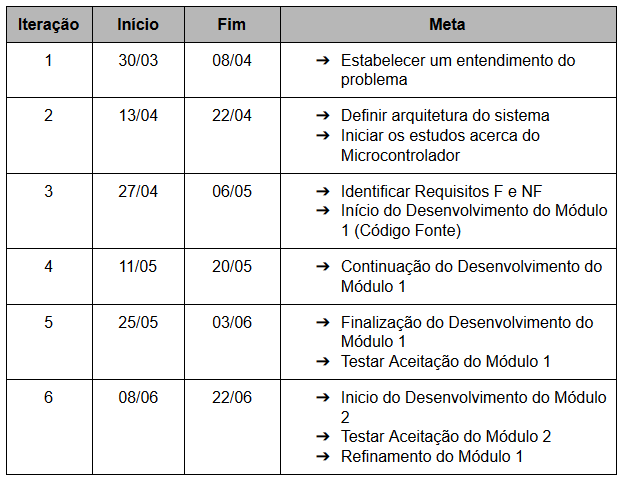
\includegraphics[width=1\textwidth]{iteracoesSOFT}
			\caption{Metas das Iterações}
			\label{iteracoesSOFT}
		\end{figure}

		No momento, finaliza-se a iteração 4 realizando a reunião de retrospectiva levantando pontos fortes e fracos, estabelecendo assim ações de melhoria para a próxima iteração. E também dar-se inicio à iteração 5 com o principal objetivo finalizar o módulo módulo 1 (Aplicação Django) completamente, incluindo os testes de aceitação.

	\subsubsubsection{Repositório de Desenvolvimento}

		O repositório de desenvolvimento na ferramenta GitHub encontra-se disponível neste link:

		\href{https://github.com/ristovao/BancadaDeTesteParaAmortecedor}{https://github.com/ristovao/BancadaDeTesteParaAmortecedor}

	\subsubsubsection{Histórias de Usuário Desenvolvidas}

		A imagem \ref{andamentoSOFT} apresentada as histórias que já foram desenvolvidas e não desenvolvidas em um \% de conclusão.

		\begin{figure}[htpb]
			\centering
			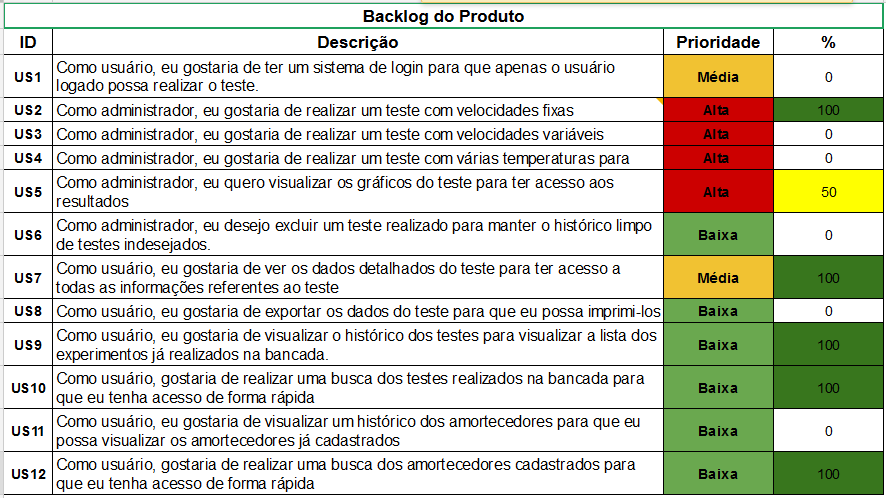
\includegraphics[width=1.1\textwidth]{andamentoSOFT}
			\caption{(\%) de conclusão das Histórias de Usuário}
			\label{andamentoSOFT}
		\end{figure}

		Ainda deve ser desenvolvido os testes de aceitação para as histórias prontas. Os critérios de aceitação são apresentados nas imagens a seguir.

		\newpage
		\begin{figure}[htpb]
			\centering
			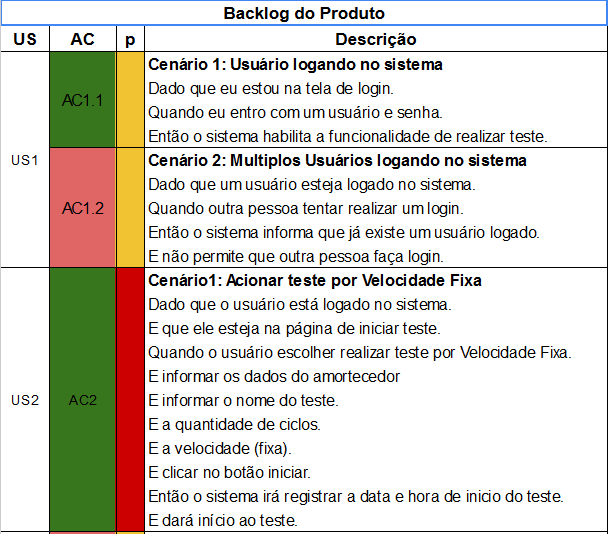
\includegraphics[width=1\textwidth]{CA01}
			\caption{Critérios de Aceitação das US - Parte 1}
			\label{CA01}
		\end{figure}

		\begin{figure}[htpb]
			\centering
			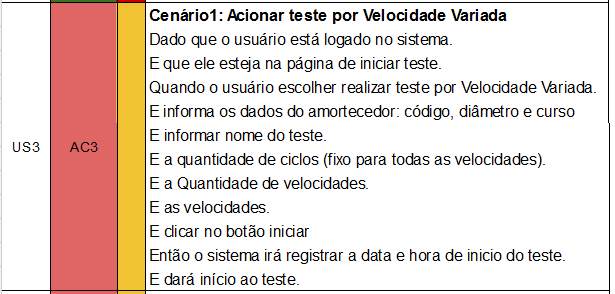
\includegraphics[width=1\textwidth]{CA02}
			\caption{Critérios de Aceitação das US - Parte 2}
			\label{CA02}
		\end{figure}

		\begin{figure}[htpb]
			\centering
			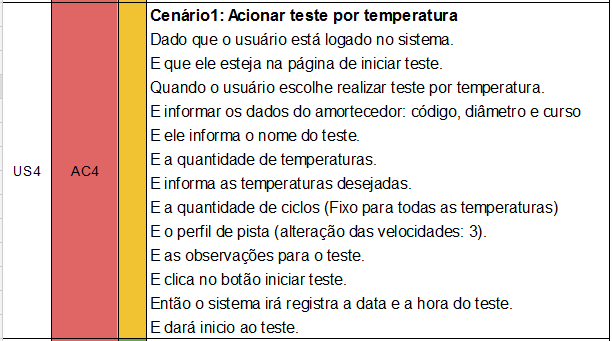
\includegraphics[width=1\textwidth]{CA03}
			\caption{Critérios de Aceitação das US - Parte 3}
			\label{CA03}
		\end{figure}

		\begin{figure}[htpb]
			\centering
			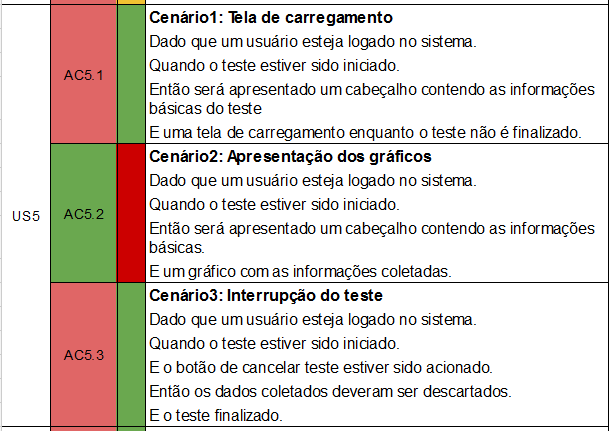
\includegraphics[width=1\textwidth]{CA04}
			\caption{Critérios de Aceitação das US - Parte 4}
			\label{CA04}
		\end{figure}

		\begin{figure}[htpb]
			\centering
			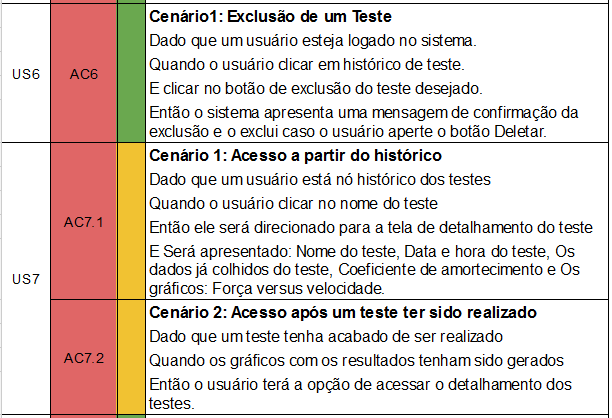
\includegraphics[width=1\textwidth]{CA05}
			\caption{Critérios de Aceitação das US - Parte 5}
			\label{CA05}
		\end{figure}

		\begin{figure}[htpb]
			\centering
			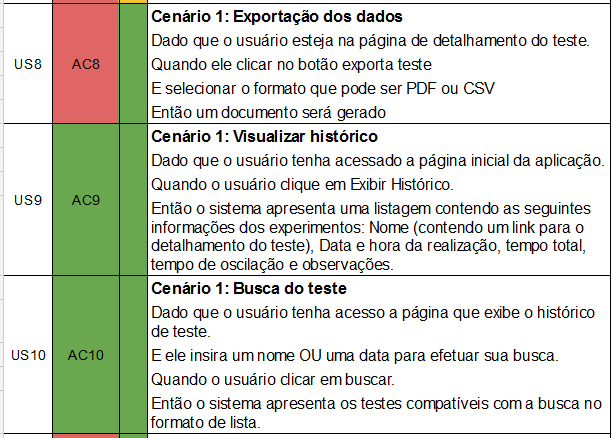
\includegraphics[width=1\textwidth]{CA06}
			\caption{Critérios de Aceitação das US - Parte 6}
			\label{CA06}
		\end{figure}

		\begin{figure}[htpb]
			\centering
			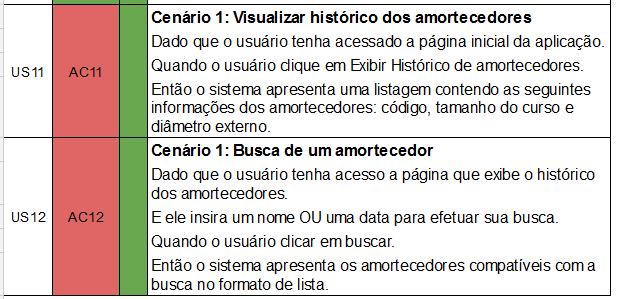
\includegraphics[width=1\textwidth]{CA07}
			\caption{Critérios de Aceitação das US - Parte 7}
			\label{CA01}
		\end{figure}


\newpage
\subsection{Ponto de Controle III}
\subsubsection{Relato do Desenvolvimento do Software}
	
	Nesta seção são descritas as atividades realizadas durante o ponto de controle III, bem como as contribuições da Engenharia de Software para o projeto Bancada e as considerações finais da Equipe.

	\subsubsubsection{Repriorização das Histórias}

		Após o ponto de controle II, as histórias de usuário foram repriorizadas. O objetivo desta nova priorização foi dar ênfase aos testes de integração necessários para o funcionamento total da bancada. Deste modo, a Figura \ref{Imagem1} apresenta a nova priorização realizada, bem como as histórias já desenvolvidas.

		\begin{figure}[htpb]
			\centering
			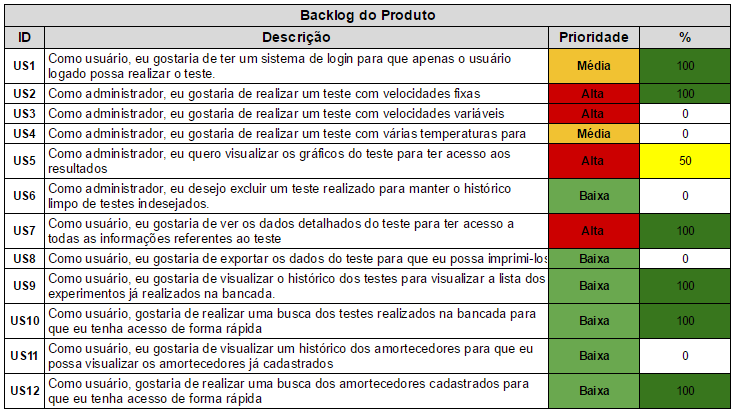
\includegraphics[width=1\textwidth]{Imagem1}
			\caption{US Repriorizadas e Desenvolvidas}
			\label{Imagem1}
		\end{figure}

		Esta nova priorização foi acordada com a Equipe de Desenvolvimento e o Membro do projeto designado como \textit{Product Owner} para o levantamento de requisitos de software (Larissa Massote – Engenharia Automotiva).

	\subsubsubsection{Replanejamento das Iterações}

		Também foi necessário adaptar o planejamento inicial previsto para as últimas semanas de desenvolvimento. O novo planejamento afetou apenas o escopo das iterações 5, 6 e 7. Seu principal objetivo foi realocar as histórias de acordo com a nova prioridade estabelecida pós ponto de controle II, apresentado no tópico anterior. A Tabela \ref{Tabela1} apresenta o novo planejamento das iterações.

		\begin{table}[htpb]
		\centering
		\caption{Planejamento das Iterações 5, 6 e 7}
		\label{Tabela1}
		\begin{tabular}{|c|c|c|c|}
		\hline
		\rowcolor[HTML]{C0C0C0} 
		{\color[HTML]{000000} \textbf{Iteração}} & {\color[HTML]{000000} \textbf{Período}} & {\color[HTML]{000000} \textbf{Histórias Alocadas}} & {\color[HTML]{000000} \textbf{(\%) de Conclusão}} \\ \hline
		{\color[HTML]{000000} 5} & {\color[HTML]{000000} 25/05 a 03/06} & {\color[HTML]{000000} US05 e US11} & {\color[HTML]{000000} 100\%} \\ \hline
		{\color[HTML]{000000} 6} & {\color[HTML]{000000} 08/06 a 17/06} & {\color[HTML]{000000} US03 e US06} & {\color[HTML]{000000} 100\%} \\ \hline
		{\color[HTML]{000000} 7} & {\color[HTML]{000000} 22/06 a 01/07} & {\color[HTML]{000000} US08 e US04} & {\color[HTML]{000000} 0\%} \\ \hline
		\end{tabular}
		\end{table}

		A execução das iterações 5 e 6 foram realizadas com sucesso e as histórias definidas para elas foram desenvolvidas e testadas. No entanto, a execução da iteração 7 não será relata neste relatório, pois o mesmo será submetido ao \textit{moodle} da disciplina no dia 24/06/2016 e o final desta iteração está planejada para o dia 01/07/2016 até 12:00.

	\subsubsubsection{Teste de Integração do Software}

		Para a integração de todos os produtos, algumas áreas foram designadas para fazer sua integração de forma conjunta, é o caso da Equipe de Engenharia de Software e Equipe de Eletrônica.
		
		O objetivo deste teste de integração era estabelecer a comunicação da aplicação, a partir de um \textit{socket} e uma porta com endereços fixos, com o microcontrolador (\textit{beaglebone black}) e iniciar a execução do teste com base nos parâmetros inseridos pelo usuário na aplicação.
		
		Para realizar está integração, foram necessários os seguintes requisitos:

		\begin{itemize}
			\item as histórias de usuário US02, US03 e US07 completamente desenvolvidas e testadas;
			\item os módulos 2 (tratamento da comunicação) e 3 (controle da entrada e saída de dados), definidos com base na arquitetura proposta, completamente desenvolvidos e testados;
			\item o teste de integração entre acionamento do motor (Equipe de Energia) com o controle da entrada e saída de dados (Equipe de Eletrônica) completamente testado e aprovado.
		\end{itemize}

		O procedimento para realização do teste de integração e apresentado na Figura \ref{Imagem2}.
		\newpage
		\begin{figure}[htpb]
			\centering
			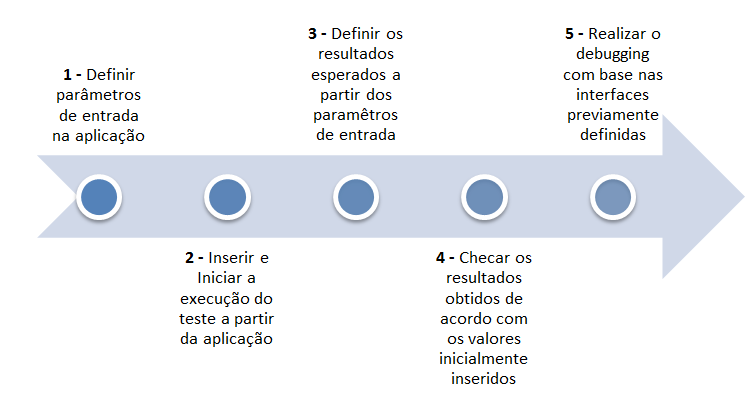
\includegraphics[width=1\textwidth]{Imagem2}
			\caption{Procedimento para realização do Teste de Integração Software-Eletrônica}
			\label{Imagem2}
		\end{figure}

		Por meio deste procedimento foi possível obter os resultados finais do teste de integração. O resultado foi dado como satisfatório quando todos os valores para o campo “resultados obtidos” estivessem de acordo com os valores de “resultados esperados”, o qual é definido com base nos parâmetros de entrada. A Figura \ref{Imagem3} apresenta o plano de teste executado.

		\begin{figure}[htpb]
			\centering
			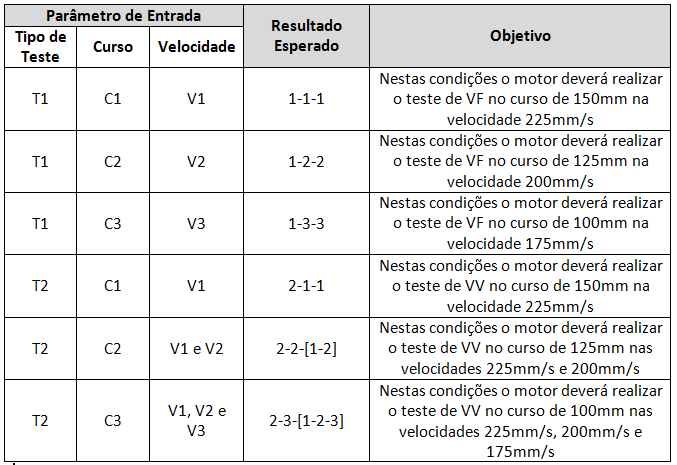
\includegraphics[width=1\textwidth]{Imagem3}
			\caption{Plano de Teste de Integração (Software-Eletrônica)}
			\label{Imagem3}
		\end{figure}

		Os resultados obtidos durante o experimento não serem inseridos neste relatório, pois não foram coletados de forma sistemática. Por fim, o resultado final do teste integração (software com eletrônica) foi dado com completo e satisfatório.

	\newpage
	\subsubsubsection{Qualidade da Aplicação}

		Existem muitas formas de definir a qualidade de uma aplicação de software. A estratégia adotada para garantir a qualidade do software aqui apresentado foi à definição e execução de testes unitários e testes funcionais.
		
		Com a utilização de teste unitário é possível garantir que as menores unidades do software (métodos) serão testadas individualmente. Quanto à utilização de teste funcional, é possível garantir que as funcionalidades da aplicação atendem os requisitos elicitados de acordo com o plano de teste elaborado.
		
		Para realizar os testes, foi necessária a utilização de algumas ferramentas específicas, conforme apresentado na Tabela \ref{Tabela2}.

		\begin{table}[htpb]
		\centering
		\caption{Ferramentas utilizadas para realização dos Testes de Software}
		\label{Tabela2}
		\begin{tabular}{|c|c|c|c|}
		\hline
		\rowcolor[HTML]{9B9B9B} 
		\textbf{Nome} & \textbf{\begin{tabular}[c]{@{}c@{}}Tipo\\   de Teste\end{tabular}} & \textbf{\begin{tabular}[c]{@{}c@{}}Ferramenta\\   ou Biblioteca\end{tabular}} & \textbf{Versão} \\ \hline
		unittest & Teste Unitário & Biblioteca (TestSuite) & 3.8 \\ \hline
		Selenium IDE Plugins & Teste Funcional & Ferramenta (Selenium IDE-Firefox) & 1.14 \\ \hline
		\end{tabular}
		\end{table}

		Atualmente, estamos no final da iteração 6. Temos um valor de aproximadamente 75\% de cobertura de teste unitário e 50\% de cobertura funcional (em relação à quantidade de critérios de aceitação definidos). Está planejado, para a iteração 7, a meta de atingir 90\% de cobertura de testes unitários e funcionais. A Figura \ref{Imagem4} apresenta um gráfico ilustrando a situação atual e a desejada.

		\begin{figure}[htpb]
			\centering
			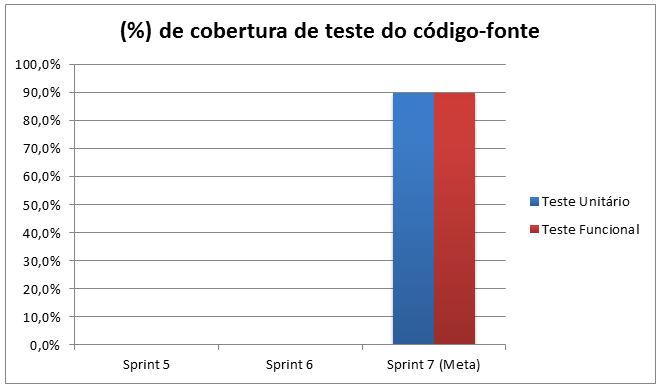
\includegraphics[width=1\textwidth]{Imagem4}
			\caption{(\%) de cobertura de teste de código-fonte}
			\label{Imagem4}
		\end{figure}

		É valido ressaltar que garantindo essa cobertura de testes para todo o código do software, alcançados sua qualidade de forma minimamente aceitável.

	\subsubsubsection{Decisões Mantidas e Abandonadas}
		
		Ao longo da execução do projeto, algumas decisões definidas inicialmente foram abandonas. Sobretudo, as decisões mantidas também foram seguidas até o final do projeto. As Figuras \ref{Imagem5} e \ref{Imagem6} apresentam todas as principais decisões mantidas, no que tange o escopo do projeto, e as decisões abandonadas respectivamente.

		\begin{figure}[htpb]
			\centering
			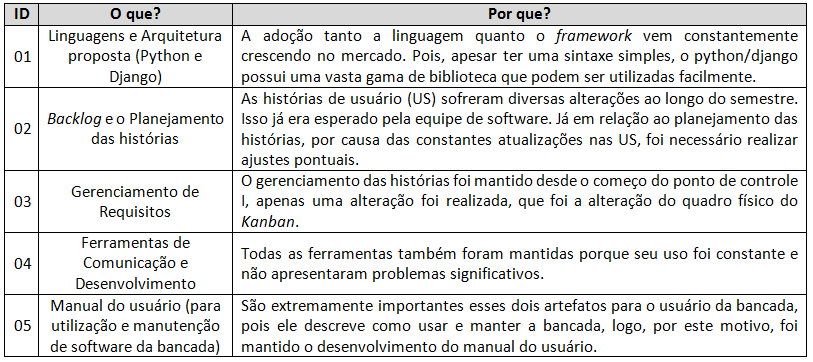
\includegraphics[width=1\textwidth]{Imagem5}
			\caption{Decisões Mantidas}
			\label{Imagem5}
		\end{figure}

		\begin{figure}[htpb]
			\centering
			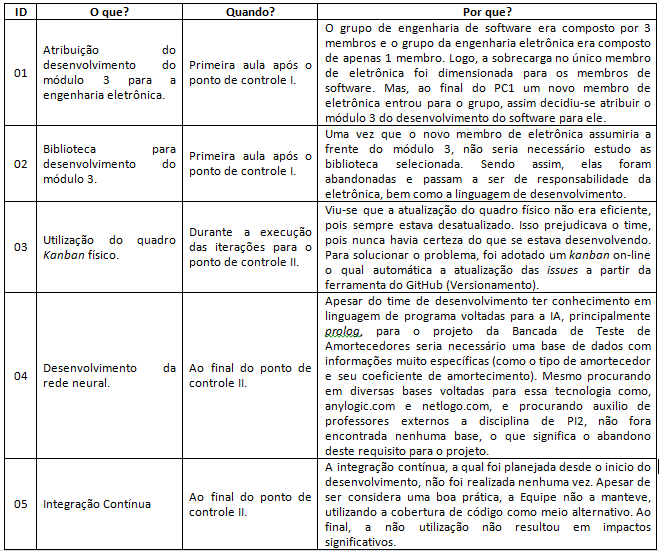
\includegraphics[width=1\textwidth]{Imagem6}
			\caption{Decisões Abandonadas}
			\label{Imagem6}
		\end{figure}

	\newpage
	\subsubsubsection{Contribuições da Engenharia de Software para o Projeto}

		As contribuições da Engenharia de Software para o projeto não tangem apenas a aplicação, mas no desenvolvimento e acompanhamento do projeto. A Equipe de Engenharia de Software possui disciplina com relação a comprimento de prazo, o que nem sempre é comum em projetos envolvendo outras disciplinas. Para solucionar esse problema, a Equipe promoveu diversos eventos comuns aos métodos ágeis como planejamento de iterações, (\textit{sprints}) revisão e retrospectiva, estimação de esforço (\textit{planning poker}) entre alguns outros.
		
		Normalmente, esses eventos eram realizados sem a percepção dos envolvidos (outras engenharias), mas que ao final sempre resultavam em um entregável a cada projeto (mecânico, eletrônico, de energia e de software), como o planejamento da iteração (\textit{backlog da sprint}), cronograma do ponto de controle (\textit{roadmap}), entre outros.
		
		A Figura \ref{Imagem7} a seguir apresentado de forma sucinta as principais contribuições da Engenharia de Software para o projeto: Bancada de Teste de Amortecedor Veicular.

		\begin{figure}[htpb]
			\centering
			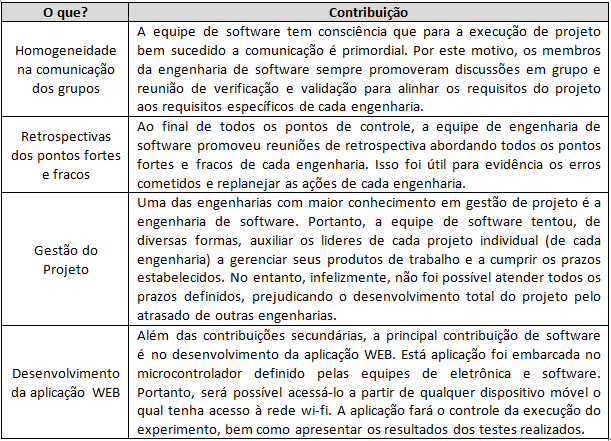
\includegraphics[width=1\textwidth]{Imagem7}
			\caption{Principais contribuições da Engenharia de Software para o projeto}
			\label{Imagem7}
		\end{figure}

	\subsubsubsection{Diagramação e Manual do Usuário}

		Alguns diagramas comuns no desenvolvimento de software tradicional foram utilizados a fim de fornecer aos desenvolvedores níveis de abstração distintos, isto é, uma visão alto nível e uma visão baixo nível. 
		
		O primeiro diagrama apresentado, Figura \ref{diagrama1}, é o Diagrama de Classes. Ele fornece uma visão das classes (Orientadas a Objetos) utilizadas na aplicação.

		\begin{figure}[htpb]
			\centering
			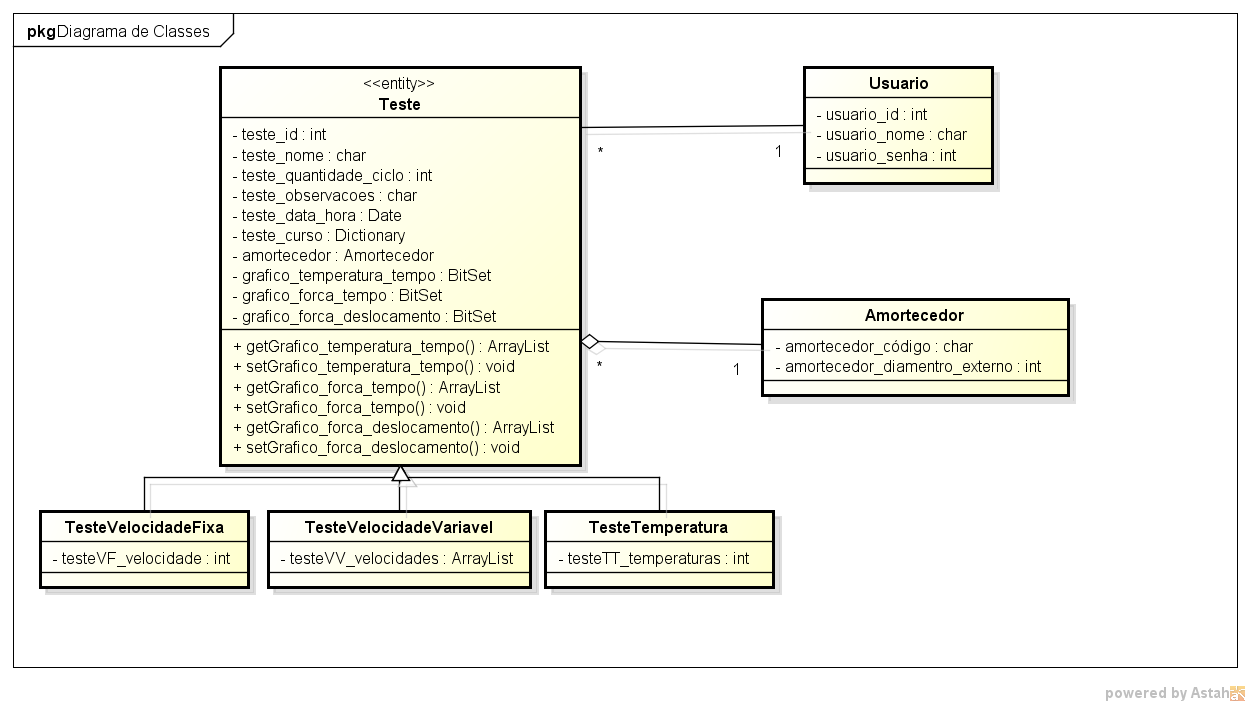
\includegraphics[width=1\textwidth]{diagrama1}
			\caption{Diagrama de Classes da Aplicação}
			\label{diagrama1}
		\end{figure}

		O segundo diagrama é o MER – Modelo de Entidade-Relacionamento, Figura \ref{diagrama2}. Ele fornece uma visão das tabelas e colunas utilizadas na base de dados da aplicação.

		\begin{figure}[htpb]
			\centering
			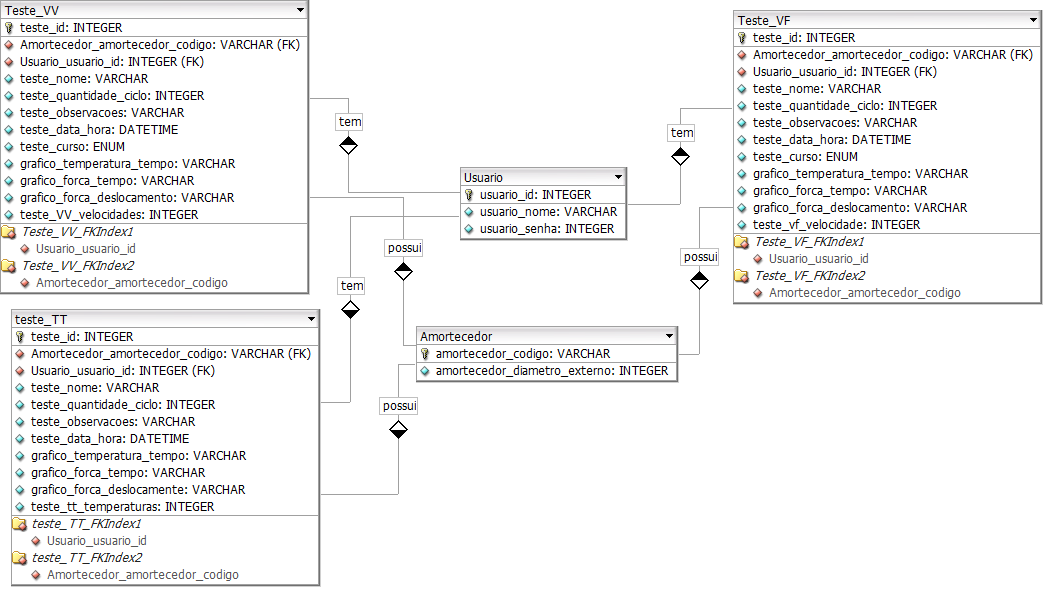
\includegraphics[width=1\textwidth]{diagrama2}
			\caption{Modelo de Entidade-Relacionamento (MER) da Aplicação}
			\label{diagrama2}
		\end{figure}

		\newpage
		O terceiro diagrama é o Diagrama de Sequencias, \ref{diagrama3}. Ele fornece uma visão lógica da arquitetura da aplicação, apresentado cada camada da arquitetura definida.

		\begin{figure}[htpb]
			\centering
			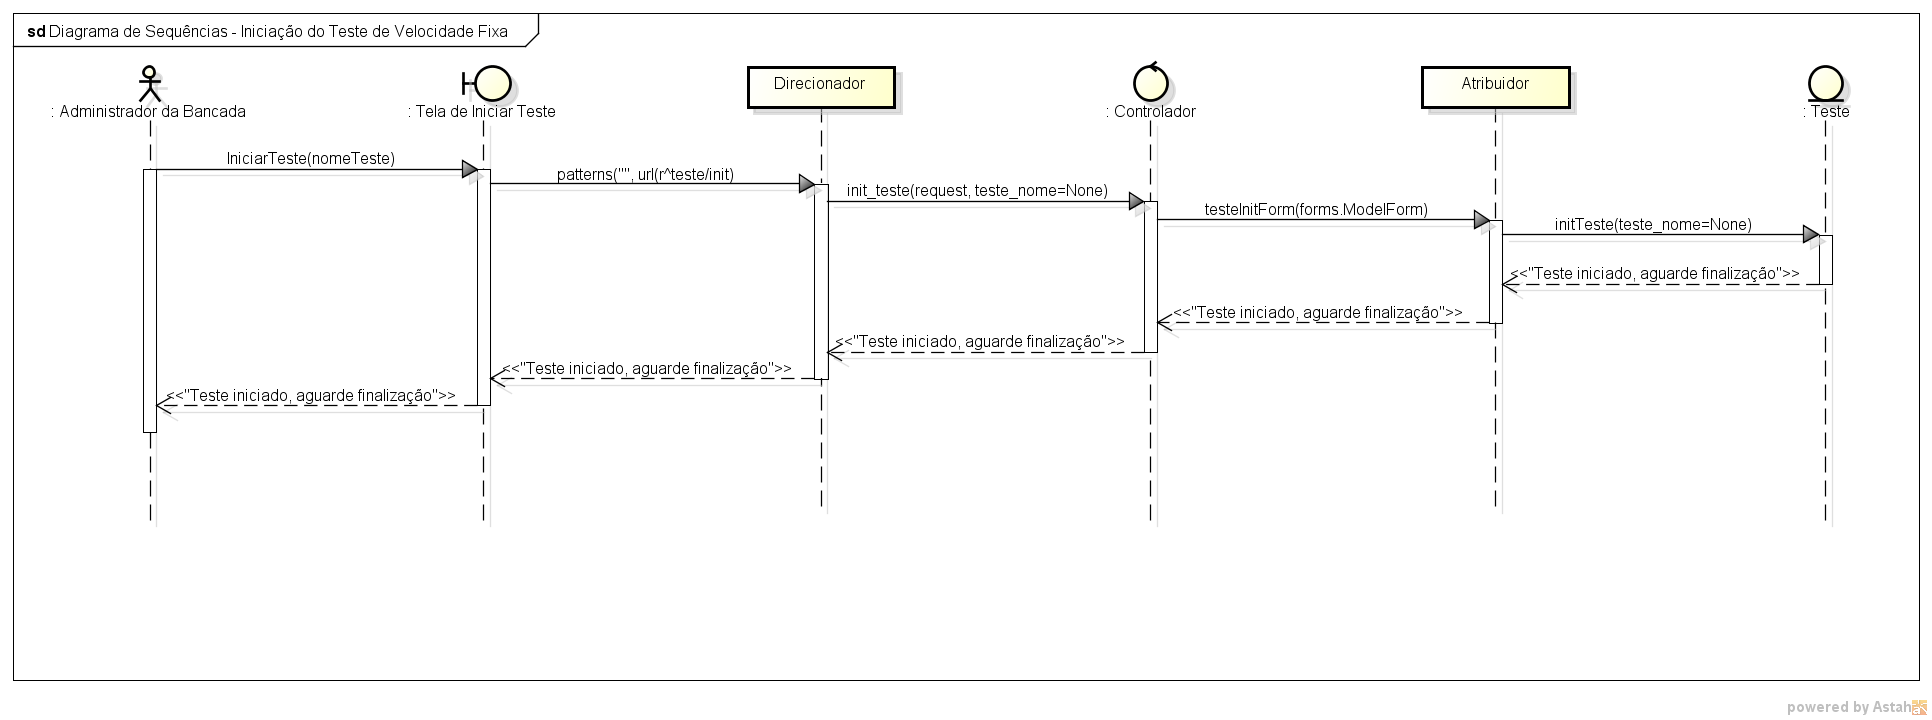
\includegraphics[width=1\textwidth]{diagrama3}
			\caption{Diagrama de Sequência da US02 da Aplicação}
			\label{diagrama3}
		\end{figure}

		\newpage
		Por fim, o quarto diagrama é a Visão Lógica da Aplicação, \ref{diagrama4}. Ele fornece uma visão lógica do caminho percorrido pela aplicação ao ser requisita uma funcionalidade qualquer do software.

		\begin{figure}[htpb]
			\centering
			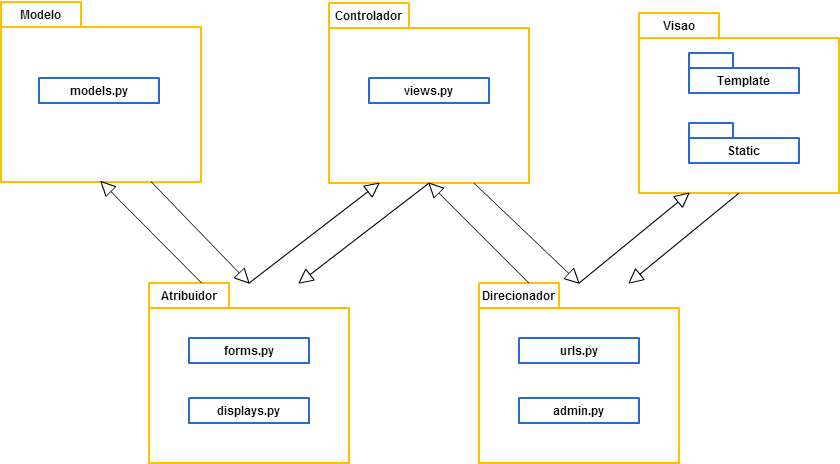
\includegraphics[width=1\textwidth]{diagrama4}
			\caption{Diagrama de Visão Lógica da Aplicação}
			\label{diagrama4}
		\end{figure}		

		Todos esses diagramas fornecem uma visão prévia, macro e micro, do software desenvolvido. Eles são inseridos no manual do usuário com o objetivo de possibilitar que outros desenvolvedores possam realizar manutenções evolutivas e corretivas na aplicação.
		
		Quanto ao manual do usuário, ele tem dois objetivos distintos, o primeiro é facilitar a manutenção do software e para isso foram anexados os diagramas da aplicação atualizados. E o segundo objetivo é fornecer informações básica para a utilização da bancada. Ou seja, fornecer um procedimento, passo-a-passo, para que o usuário consiga utilizar a bancada sem dificuldades.
		
		Este manual é composto de uma área técnica apresentando todas as informações técnicas (de todas as engenharias envolvidas no desenvolvimento da aplicação) necessárias para operação e manutenção da bancada, e uma área não-técnica, o qual apresenta informações usuários para utilização da bancada por um leigo.
		
		Para a área de software, foram inseridas no manual os diagramas desenvolvidos e o procedimento de execução da bancada.
		
		O manual é um documento não anexado neste relatório, e será apresentado durante a utilização da bancada no dia 01/07/2016.

	\subsubsubsection{Considerações Finais da Equipe de Engenharia de Software}

		O projeto de software teve alguns atrasos que foram significativos para a aplicação, mas que não afetaram a qualidade do software ao final. Sobretudo, todas as funcionalidades identificadas foram desenvolvidas e testadas e apresentaram-se úteis para a utilização da bancada, após a validação final com o \textit{Product Owner} (membro do projeto – Larissa Massote).
		
		A Equipe de Engenharia de Software acredita que o objetivo final do projeto de Software foi alcançado com sucesso, contribuindo de forma positiva para o projeto final: Bancada de Teste de Amortecedores Veicular. 